%!xelatex = 'xelatex --halt-on-error %O %S'

\documentclass{thuemp}
\usepackage{url}
\usepackage{lipsum}  % 生产假书乱文的包,实际使用时可去掉
% \usepackage{graphicx}
\usepackage{hyperref}
\begin{document}

% \enlargethispage{-0.2cm}
% 标题,作者
\emptitle{脑-芯融合:神经形态芯片与脑控无人系统的应用}
\empauthor{秦华谦}{王涛老师}

% 奇数页页眉 % 请在这里写出第一作者以及论文题目
\fancyhead[CO]{{\footnotesize 秦华谦: 脑-芯融合:神经形态芯片与脑控无人系统的未来应用}}


%%%%%%%%%%%%%%%%%%%%%%%%%%%%%%%%%%%%%%%%%%%%%%%%%%%%%%%%%%%%%%%%
% 关键词 摘要 首页脚注
%%%%%%%%关键词
\Keyword{神经形态计算芯片, 脑机接口技术, 无人系统前景}
\twocolumn[
\begin{@twocolumnfalse}
\maketitle

%%%%%%%%摘要
\begin{empAbstract}
  在科学技术不断发展的背景下,人们对脑机接口和无人系统的关注和研究逐渐增加。其中,新兴的神经形态芯片技术,凭借其模拟人脑神经元功能和结构的特性,为无人系统的脑控技术发展开辟了新的可能性和机遇。
  
  文章首先介绍了神经形态芯片的基本工作原理。接着,分析了当前脑控无人系统的状况和面临的挑战。然后,文章着重展望了神经形态芯片在医学和军事领域的潜在应用,尤其是在医学领域,神经形态芯片有可能促进脑机接口技术的进步,从而改善失能患者的生活质量。在最后的结论部分,文章强调了神经形态芯片在脑控无人系统中的潜力和未来应用前景。
  
  对于未来的研究方向,文章建议对神经形态芯片的设计和制造技术进行进一步的改进,以提升其计算和处理能力,同时开发更先进的脑控无人系统应用。此外,也需要解决与脑控技术相关的伦理、安全和隐私问题,以保证其应用的合理性和可行性。
\end{empAbstract}

%%%%%%%%英文标题、作者、摘要、关键词
\emptitleEn{Brain-Chip Fusion: Applications of Neural Morphology Chips and Brain-Controlled Unmanned Systems}
\empauthorEn{Huaqian Chin}{Prof. Wang Tao}
\KeywordEn{Neuromorphic Computing Chips, Brain-Computer Interface Technology, Prospects for Unmanned Systems}

\begin{empAbstractEn}
  In the context of the continuous development of science and technology, people's attention and research on brain-computer interface and unmanned systems have gradually increased. Among them, the emerging neuromorphic chip technology, by virtue of its characteristics of simulating the function and structure of human brain neurons, has opened up new possibilities and opportunities for the development of brain control technology for unmanned systems.
  
  The article first introduces the basic working principle of the neuromorphic chip. Then, the current status and challenges of mind-controlled unmanned systems are analyzed. Then, the article focuses on the potential application of neuromorphic chips in the medical and military fields. Especially in the medical field, neuromorphic chips may promote the advancement of brain-computer interface technology, thereby improving the quality of life of disabled patients. In the final concluding section, the article highlights the potential and future application prospects of neuromorphic chips in brain-controlled unmanned systems.
 
  For future research directions, the article recommends further improvements to the design and manufacturing technology of neuromorphic chips to enhance their computing and processing capabilities, while developing more advanced brain-controlled unmanned system applications. In addition, ethical, security and privacy issues related to brain control technology also need to be resolved to ensure the rationality and feasibility of its application.
\end{empAbstractEn}

% \pagebreak % 在摘要和脚注之间插入分页避免重合
% \enlargethispage{-2cm}
%%%%%%%%首页角注,依次为实验时间、报告时间、学号、email
\empfirstfoot{2023-5-30}{2023-5-30}{21312683}{qinhq5@mail2.sysu.edu.cn}
\end{@twocolumnfalse}
]
%%%%%%%%!首页角注可能与正文重叠,请通过调整正文中第一页的\enlargethispage{-3.3cm}位置手动校准正文底部位置:
%%%%%%%%%%%%%%%%%%%%%%%%%%%%%%%%%%%%%%%%%%%%%%%%%%%%%%%%%%%%%%%%
%  正文由此开始
\wuhao 
%  分栏开始

\section{引~~言}
% \enlargethispage{-3.3cm}
科技进步的浪潮中,脑机接口和无人系统的研究已经取得了显著成果。脑机接口技术实现了人类与计算机或机器的直接交流,而无人系统则通过自主行动,无需人工干预,完成各类任务。神经形态芯片,这项新兴技术,提供了一种全新的视角和机遇,推动了脑控无人系统的发展,并展示出巨大的潜能。

神经形态芯片是一种仿生的计算芯片,模拟了大脑神经元的结构和功能。相比传统的计算机芯片,它能更有效地处理复杂信息,具备学习和适应的能力,这使得它在脑控无人系统中具有巨大的应用潜力,实现更为智能化和自主化的操作。

本研究的目标是深入探讨神经形态芯片在脑控无人系统中的应用,同时分析其在医学、军事等领域的发展前景。我们将从解析神经形态芯片的基本原理开始,介绍它如何模拟神经元功能及其优点。然后,我们将概述脑控无人系统的现状和面临的挑战,以理解神经形态芯片能够解决的问题。我们还将介绍神经形态芯片在脑控无人系统中的应用案例,包括单个无人车系统、多无人车系统、无人船和太空飞行器等。此外,我们将讨论神经形态芯片在医学和军事领域的可能应用,并对可能涉及的伦理和社会问题进行讨论。

我们希望通过对这些主题的研究和分析,能够深化对神经形态芯片在脑控无人系统中应用的理解,并为其未来的研究和发展提供参考。神经形态芯片在脑控无人系统中的应用展示了令人期待的前景,将进一步推动无人系统技术的进步,并引领我们步入一个更智能和自主的未来。

\section{神经形态芯片的基本原理}

\begin{figure}[h]
	\centering
    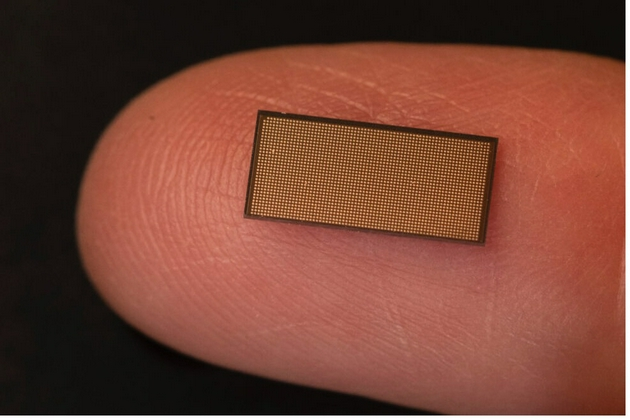
\includegraphics[width=0.8\linewidth]{./img/yte_sjxp.jpg}
    \caption{英特尔研发的神经芯片: $31mm^2$容纳100万人工神经元} 
\end{figure}

\subsection{神经形态芯片概述}

神经形态芯片是一种受到人脑神经系统启发设计的芯片,其结构和功能模拟大脑神经元。这与传统计算机芯片有所不同,因为神经形态芯片利用模拟神经元和神经元间连接的方式进行信息处理,其处理方式更接近于人脑。

\subsection{模拟神经元功能}

\subsubsection{神经元组成仿生}
神经形态芯片的基础构成单元是模拟神经元的神经元模拟器,这种模拟器可以模拟生物神经元的基本功能。通常,神经元模拟器由多个子单元组成,包括模拟膜电位、突触传输和神经递质释放等功能的部分。这些子单元模拟神经元内外电位变化以及突触间的信号传导,从而复制了神经元的兴奋和抑制过程。

\begin{figure}[h]
	\centering
    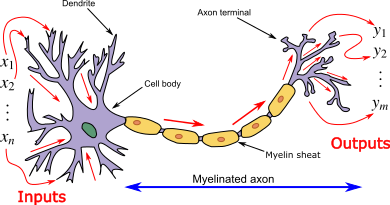
\includegraphics[width=0.8\linewidth]{./img/sjy.png}
    \caption{神经元}
\end{figure}

\subsubsection{神经形态芯片的连接结构}
神经形态芯片模拟了神经元之间的连接结构,从而实现了神经网络的建立。通常,神经元间的连接采用可调的突触权重,这种权重可以调整神经元之间信号传递的强度和方向。通过这种可调的突触权重,神经形态芯片具备了学习和适应外部输入的能力,并能形成动态的神经网络拓扑结构。

\subsubsection{神经形态芯片的并行处理能力}
通常,神经形态芯片会利用并行计算的策略来增强信息处理的能力。每个神经元模拟器都具备同时处理众多输入信号的能力,且能在极短的时间里产生相关的输出。借助于并行的计算进行的同时,神经形态芯片有能力迅速地处理复杂的信息,实现神经网络计算的高效性。

\subsubsection{学习和适应能力}
神经形态芯片具有学习和调整自身的能力,能够根据外部输入的变动对神经网络的连接权重进行改变。此种学习和自我调节的能力让芯片有可能自我调整其功能,以满足各种任务和环境的需求。通过这种学习和自我调节,神经形态芯片能更有效地模拟人脑的认知和决策过程。

\subsection{优势}
神经形态芯片的基础理论使其具备模拟和执行人脑神经功能的能力,为脑控制无人系统提供了强大的计算实力。通过融合神经形态芯片与脑机接口技术,无人系统能与人脑直接交流和互动,达到更智能、自主的操作和决策。这种依赖神经形态芯片的脑控制无人系统具有巨大的应用潜力,可以运用于独立无人车系统、多无人车系统、无人船以及空间飞行器等领域。

\section{脑控无人系统的现状和挑战}
\subsection{脑机接口技术概述}
脑机接口技术(Brain-Computer Interface, BCI)是一种使大脑活动信息转换成机器可解码的形式的方法。利用脑电图(EEG)和功能磁共振成像(fMRI)等工具,我们能够获取人脑中的电信号以及血液中的氧合水平等生理数据。经过数据处理和模式检测算法,这些信号可以与计算机或无人系统进行有效沟通,从而控制无人系统通过思维指令进行操作。

\subsection{无人系统的发展和应用}
无人系统在军事、航天、医疗和物流等领域都有着广阔的使用范围。无人驾驶汽车、无人飞行器、无人船等自主执行任务的无人系统具备在高效、精准及危险环境下操作的可能性。尽管随着科技的进步,无人系统在自我决策、智能化和灵活性上已有所提升,但仍需面临一些挑战。

\subsection{脑控无人系统的挑战和限制}
虽然脑机接口和无人系统各自已取得显著的进步,但要将两者融合形成脑控无人系统,仍需克服一些困难和局限。诸如信号解析度、实时响应、用户训练以及适应性,还有伦理和隐私问题等,都是脑控无人系统所需面临的挑战。战胜这些困难将成为脑控无人系统发展的关键推动力,并促使其在各种领域得到更广泛的应用。

\begin{figure}[h]
	\centering
    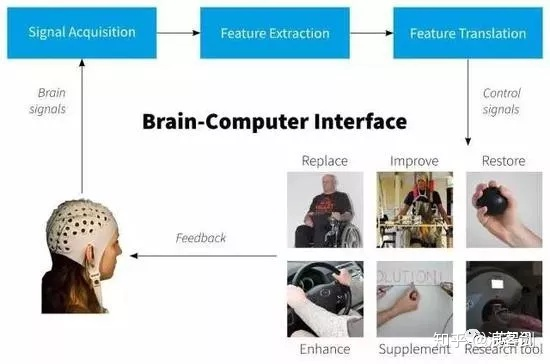
\includegraphics[width=0.8\linewidth]{./img/njjk-lch.jpg}
    \caption{脑控无人系统流程概览}
\end{figure}

\subsubsection{信号分辨率和准确性}
脑控无人系统的运作需要准确捕捉并解析大脑信号,再将这些信号转化为可执行的命令。然而,现有的脑机接口技术在信号解析度和精度上仍有一定的短板。因素如大脑信号中的噪声、干扰以及对特定动作和意愿的辨识精度等问题,都在阻碍脑控无人系统的精确性和可信度。

\subsubsection{实时性和延迟}
对脑控无人系统而言,快速地响应并执行来自大脑的指令是至关重要的,这就要求系统能够及时解读大脑信号并将其转化为具体行为。但是,在收集信号、处理信号以及传递指令的各个环节中出现的时间延迟都可能对系统的实时反应性产生负面影响。因此,缩短这种延迟,并提升信号处理与传输的效能是脑控无人系统必须面对和解决的问题。

\subsubsection{用户训练和适应性}
为了确保脑控无人系统能够有效运行,用户需要进行一定的训练和适应过程,以在其大脑信号和系统操作间建立稳定的映射关系。用户的训练时间长短以及效果的好坏直接决定了脑控无人系统的实用性和用户的体验感。因此,如何让用户的训练过程更为便捷,以及提升用户适应系统的能力,是一个需被解决的关键问题。

\subsubsection{伦理和隐私问题}
由于脑控无人系统需要获取并利用个体的大脑信号,因此涉及到伦理和隐私的问题。确保用户隐私和个人数据的安全,以及保证系统的合规使用和道德行为,是这个领域需要重视并解决的问题。

\section{神经形态芯片在脑控无人系统中的应用案例}
神经形态芯片在脑控无人系统中的应用范围包括但不限于单个无人驾驶系统、多个无人驾驶系统、无人船以及太空飞行器等。由于神经形态芯片具有智能模拟和自我适应的能力,它使得脑控无人系统能以更智能、自主的方式执行任务,并实现与人脑的精准交流和互动。这些应用实例为脑控无人系统的未来发展展示了巨大的应用潜力。

\subsection{单无人车系统}
在单个无人驾驶系统中,神经形态芯片的应用能显著提升系统的智能化和自主化水平。通过与脑机接口技术的结合,神经形态芯片能解读驾驶员的意愿和指示,并将其转变为无人车的行动和决策。比如,驾驶员可以通过思维来控制无人车的行驶、转向和停止等操作。此外,神经形态芯片的学习和适应能力还能使无人车从驾驶员的行为中吸取经验并改善其驾驶策略,从而提升驾驶的安全性和效率。

\subsection{多无人车系统}
在多无人驾驶系统中,神经形态芯片的使用可以促进车辆间的协同操作和智能决策制定。每个装有神经形态芯片的无人车都能实时感知周围环境、解析其他车辆的行动和意图,并在此基础上进行决策和规划。通过神经形态芯片与无线通信的联接,多个无人车能实现分布式的智能合作,从而共同完成如交通调度、自动驾驶车队等复杂任务。

\subsection{无人船}
神经形态芯片在无人船系统中的运用能够增强船只的自主导航能力。搭载有神经形态芯片的无人船可以模拟并学习在海洋环境中的感知和决策流程。通过结合脑机接口技术,无人船能够根据船员的意愿和指令,自主地完成航行、避障、航线规划等各类任务。除此之外,神经形态芯片还能够分析各类海洋数据,如海流、波浪和水质等,为无人船提供更为精确的导航信息和环境适应性。

\subsection{空间飞行器}
在空间飞行器中,神经形态芯片的应用可以提高飞行器的智能、自主和自适应能 力。通过与脑机接口技术结合,神经形态芯片能够感知宇航员的意图和生理状态,对飞 行器进行精确控制和操作。此外,神经形态芯片可以模拟和学习宇宙环境中的感知和 决策过程,为飞行器提供更强大的自主导航和任务执行能力。例如,飞行器可以通过脑 控实现姿态调整、轨道控制和任务执行等。

\section{神经形态芯片在医学和军事领域的应用展望}
\subsection{医学领域的应用展望}
\subsubsection{脑机接口和假肢控制}
神经形态芯片能与人脑互动,使脑机接口技术在医疗领域得以应用。通过脑控假肢,神经形态芯片能解读大脑信号,让身体残障者能够通过思维来操控假肢的动作,从而实现肢体功能的复原或替代。这对于失去肢体的人来说,无疑是一项具有颠覆性的技术。

\subsubsection{神经疾病治疗}
神经形态芯片能模拟并调整神经系统的功能,从而为神经疾病的治疗开辟新的途径。比如说,对于帕金森病患者,神经形态芯片可以通过刺激特定的神经元来缓解病状。另外,神经形态芯片还可被用于通过脑电刺激来治疗抑郁症和癫痫等神经系统疾病,从而为病患提供更为精准和有效的治疗方案。

\subsection{军事领域的应用展望}
\subsubsection{军事操作和指挥}
应用脑控技术和神经形态芯片,士兵有能力借助思维来操纵军用装备和武器系统,这将极大地提升军事行动的速率和精确性。除此之外,神经形态芯片具备实时跟踪士兵的身体和心理状态的能力,这为军队指挥官提供了重要的数据来源,助力他们制定出更精准的策略。

\subsubsection{士兵训练和增强}
神经形态芯片的利用也能在军人的培训和增能上发挥关键角色。依靠与脑机接口的协同,军人能够通过思维进行模拟训练,以此提升他们的反应迅速性、目标定位能力以及战术决策力。而且,神经形态芯片也可以用于提升军人的认知能力,从而增强他们的专注力、记忆力以及学习能力。

\subsection{小结}
总的来说,神经形态芯片在医疗和军事领域具有巨大的潜力。在医疗领域,它们可能开创新的治疗方法,使病患重新获得丧失的功能,同时提升他们的生活品质。而在军事领域,通过应用神经形态芯片,无人系统的操作效能和准确性将得到显著提升,这将对军事行动和军事训练产生深远影响。然而,这些应用同样伴随着伦理、隐私和安全等问题的出现,因此在推动应用的同时,也需要认真对待并解决这些问题。

\section{神经系统芯片与人工智能的结合}
在未来的设想中,神经形态芯片和人工智能技术的结合可以带来高度智能化的脑控无人系统。随着科技的发展,我们能期待神经形态芯片在模拟复杂神经网络的能力更上一层楼,同时人工智能技术也为无人系统提供了更强大的计算和决策支持。以下是这样一个设计概念的具体方向:

\begin{itemize}
	\item 增强的感知和决策能力:神经形态芯片可以模拟大脑的感知和决策机制,能够准确地处理和理解来自环境的信息,通过与大脑的交互以及利用深度学习、强化学习等人工智能技术进行复杂的决策。这意味着无人系统能具有更快、更精确的感知和决策能力,使其能够应对各种复杂的环境和任务。
	\item 自我学习和适应:脑控无人系统可以结合神经形态芯片和人工智能技术实现自我学习和适应。神经形态芯片可以模仿人脑的学习过程,通过感知环境变化和与人脑交互来优化自身的行为。而人工智能技术可以利用大数据和强化学习算法,引导系统的学习过程,使其能够自主地根据不同的任务和环境进行调整和适应。
	\item 有效的协作和交互:脑控无人系统可以利用神经形态芯片和人脑进行精确的交流和互动。通过脑机接口技术,系统可以解码人脑的意图和指令,并将这些信息转化为具体的行动和操作。同时,系统还可以通过感知人脑的反馈信号,实现双向的信息传递和协同操作。这样一来,人和脑控无人系统之间可以实现高度的交互和合作,从而提高任务执行的效率和准确性。
\end{itemize}

\section{应用假设}
\subsection{神经形态芯片在假肢控制中的一个具体应用方案和使用方法}

\begin{figure}[h]
	\centering
    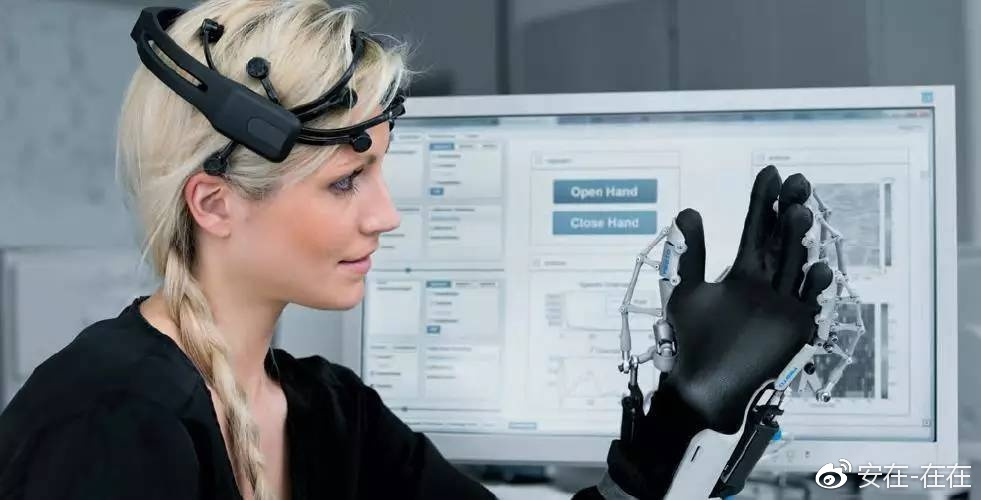
\includegraphics[width=0.8\linewidth]{./img/njjk-jzh.jpeg}
    \caption{脑机接口控制假肢效果图}
\end{figure}

{\heiti 神经形态芯片选择:}
\begin{itemize}
	\item 研究目的:明确目标脑区的特点和需要解码的大脑信号类型,例如运动皮质的神经元活动和肢体运动信号。
	\item 芯片功能:选择具有合适的功能和特性的神经形态芯片,如能够采集和解码大脑信号、控制假肢运动的芯片。
\end{itemize}

{\heiti 植入手术:}
\begin{itemize}
	\item 手术规划:与神经外科医生和团队合作,制定患者个体化的手术方案,包括目标区域的定位和手术路径的规划。
	\item 手术操作:在手术室中进行植入手术,确保严格的无菌操作和精确的芯片定位。根据预定方案,将神经形态芯片植入患者的大脑目标区域。
\end{itemize}

{\heiti 连接和调节:}
\begin{itemize}
	\item 连接设备:使用导线或无线技术,将神经形态芯片与外部假肢和控制设备或调节器连接。确保连接的稳定性和可靠性。
	\item 参数调节:根据患者的需求,通过外部设备或调节器调节神经形态芯片的参数。这包括神经信号的采集频率、解码精度和控制信号的生成等参数的调整。
\end{itemize}

{\heiti 使用和监测:}
\begin{itemize}
	\item 功能评估:使用专门的评估工具对患者的功能进行评估,包括肢体运动、精细动作和假肢控制等方面。
	\item 生活质量评估:采用相关的生活质量评估工具评估患者的生活质量,包括日常活动、自我照顾能力和社交功能等方面。
\end{itemize}

{\heiti 调整和优化:}
\begin{itemize}
	\item 定期随访:定期与患者进行随访,评估使用效果和患者反馈。根据随访结果,确定是否需要调整参数设置和训练策略。
	\item 个体化调节:根据患者的个体差异和需求变化,调整神经形态芯片的参数和控制策略,以获得最佳的使用效果和患者满意度。
\end{itemize}

\section{结论与展望}
\subsection{结论}
神经形态芯片,这种仿生神经系统的技术,为脑控无人系统开启了崭新的篇章。这种芯片具备模仿人脑神经系统的独特能力,通过与脑机接口的融合,它能实现与人脑的深度交互,让无人系统具备更强的智能性、自主性和适应能力。

在医学领域,神经形态芯片的应用展现出巨大的潜力,预示着脑机接口、假肢控制以及神经疾病治疗等领域的未来可能将发生颠覆性的变革。例如,它能帮助脑机接口技术得到进一步发展,让人们通过思维来控制假肢,极大地提高了假肢的使用体验;同时,它也可能通过刺激神经系统,为治疗帕金森病、癫痫、抑郁症等神经疾病提供更为精准的手段。

在军事领域,神经形态芯片的应用前景更是广阔。通过神经形态芯片,士兵能通过意念控制军事设备,这将大大提升军事操作的速度和准确性。此外,通过监测士兵的生理和心理状态,这种技术还可以为指挥官提供重要的决策信息。同时,士兵也可以通过脑控技术进行模拟训练,提升反应速度、战术决策能力等。

当然,虽然神经形态芯片为我们提供了无尽的可能性,但同时也引发了一系列的伦理、隐私和安全问题。因此,在未来的研究和应用中,我们需要密切关注并妥善处理这些问题。

\subsection{展望}
神经形态芯片在脑控无人系统中的应用确实充满了巨大的可能性,但这并不意味着我们可以忽视其面临的挑战和问题。在实现这些广阔前景的过程中,我们首先需要突破在设计和制造神经形态芯片的技术难题,实现高性能和高可靠性的芯片制造。其次,信号处理和分析算法的改进也是关键,需要提高信号的分辨率和实时性,以便更准确地解读脑信号。

而且,我们不能忽视涉及伦理、隐私和安全的问题。这些挑战必须得到妥善处理,以确保用户的权益和数据安全得到保护。在此过程中,可能需要我们进行深入的伦理讨论,建立相关的法规和规范,以及开发高效的安全防护技术。

展望未来,我们有理由期待神经形态芯片在脑控无人系统中扮演更重要的角色。随着技术的不断突破,未来可能会出现更先进、更高效的神经形态芯片,可以更好地模拟和复制人脑的复杂神经网络,从而实现更精确的脑控和交互。

同时,结合人工智能和机器学习等其他领域的技术,我们可以进一步提升脑控无人系统的性能和应用范围。比如,人工智能和机器学习可以帮助无人系统进行自主学习和决策,以适应复杂的任务和环境。

无论是在医学还是军事领域,神经形态芯片的应用前景都非常广阔。虽然目前还面临一些挑战和问题,但我们有理由相信,随着科技的进步和创新,神经形态芯片有可能引领我们进入一个更智能、自主和高效的无人系统时代。
\cite{崔翯2023脑机接口概论}



%%%%%%%%%%%%%%%%%%%%%%%%%%%%%%%%%%%%%%%%%%%%%%%%%%%%%%%%%%%%%%%%
%  参考文献
%%%%%%%%%%%%%%%%%%%%%%%%%%%%%%%%%%%%%%%%%%%%%%%%%%%%%%%%%%%%%%%%
%  参考文献按GB/T 7714-2015《文后参考文献著录规则》的要求著录. 
%  参考文献在正文中的引用方法:\cite{bib文件条目的第一行}

\renewcommand\refname{\heiti\wuhao\centerline{参考文献}\global\def\refname{参考文献}}
\vskip 12pt

\let\OLDthebibliography\thebibliography
\renewcommand\thebibliography[1]{
  \OLDthebibliography{#1}
  \setlength{\parskip}{0pt}
  \setlength{\itemsep}{0pt plus 0.3ex}
}

{
\renewcommand{\baselinestretch}{0.9}
\liuhao
\nocite{*}
\bibliographystyle{gbt7714-numerical}
\bibliography{./TempExample}
}



\end{document}

